\section*{Introduzione}
Il corso di Architetture Avanzate dei Calcolatori si prefigge lo scopo di fornire una vista sulle più recenti architetture avanzate dei calcolatori, introducendo i meccanismi base delle micro-architetture che si possono ritrovare nei moderni microprocessori, ed infine fornire le ragioni dietro alle tecniche adottate nelle architetture dei computer.
\section{Pipelining}\label{capitolo1}
\subsection{Concetti base}
Definiamo prima di tutto quali sono le principali caratteristiche dell'architettura MIPS partendo dalla definizione delle istruzioni utilizzate da questi calcolatori calcolatori.
Esistono due tipi di istruzioni le CISC e le RISC; le istruzioni di tipo \textbf{CISC} (\emph{Complex Instruction Set Computer}) sono un set di istruzioni esteso che permettono ai processori di eseguire operazioni molto complesse come somme tra operandi caricati direttamente dalla memoria centrale, le istruzioni \textbf{RISC} (\emph{Reduced Instruction Set Computer}), invece, sono istruzioni semplici che possono essere eseguite in un unico ciclo di clock e ottimizzate per le performance sulle CPU CISC.
Le architetture RISC sono anche dette architetture di tipo \emph{LOAD/STORE}, in quanto le istruzioni non accedono direttamente ai dati in memoria ma accedono ai dati contenuti in registri del processore, solo due istruzioni permettono l'accesso alla memoria principale, queste due istruzioni sono: 
\begin{itemize}
\item \textbf{load} che carica i dati dalla memoria ai registri.
\item \textbf{store} che sposta i dati dai registri alla memoria.
\end{itemize}
Un'altra caratteristica fondamentale per le architetture RISC è l'utilizzo della \emph{Pipeline} una tecnica di ottimizzazione basata sull'esecuzione sovrapposta di molteplici istruzioni sequenziali.
\subsubsection{Reduced Instruction Set nei processori MIPS}
Vediamo ora quali sono le diverse istruzioni di tipo RISC e come sono rappresentate nel calcolatore
\paragraph{Istruzioni ALU}
Vediamo innanzitutto le istruzioni di somma ovvero quelle eseguite dalla ALU. Queste possono essere di due tipi,
Una istruzione di tipo \emph{R-Format} è un istruzione che prende in considerazione due registri, tale tipo di operazione è applicabile solo alle istruzioni \texttt{add} di tipo registro-registro. Esistono poi le \texttt{addi} che viene chiamata anche somma \emph{immediata} in quanto avviene tra un registro ed un valore costante. Tale tipo di istruzione è del tipo \emph{I-Format}.
Lo pseudo codice assembly  delle due istruzioni è mostrato qui di seguito, inoltre possiamo anche vedere come vengono svolte le operazioni.
\begin{verbatim}
add  $s1, $s2, $s3      # $s1 <- $s2 + $s3
addi $s1, $s2, 4        # $s1 <- $s2 + 4
\end{verbatim}
In \figurename\,\ref{fig:regALU} vediamo come è suddivisa un'istruzione di tipo \emph{R-Format} 
\begin{figure}[htb]
\centering
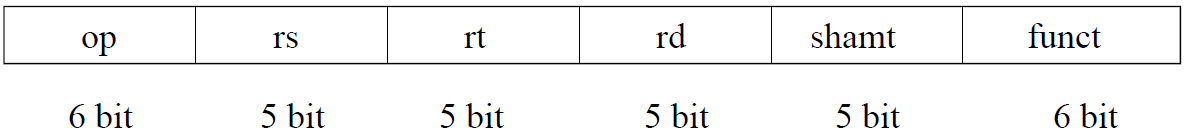
\includegraphics[scale=0.4]{img/regALU.png}
\caption{Esempio di istruzione ALU di tipo R-Format}\label{fig:regALU}
\end{figure}
I diversi campi indicano rispettivamente:
\begin{description}
\item[op] identifica il tipo di istruzione ALU da eseguire
\item[rs] indica il registro nel quale è contenuto il primo operando
\item[rt] indica il registro nel quale è contenuto il secondo operando
\item[rd] indica il registro di destinazione
\item[shamt] sta ad indicare i bit di shift amount
\item[funct] identifica i diversi tipi di istruzione
\end{description}
\begin{figure}[htb]
\centering
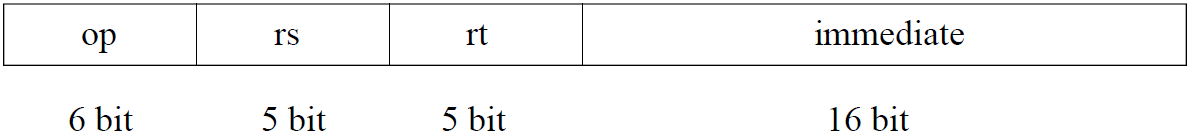
\includegraphics[scale=0.4]{img/ALUdir.png}
\caption{Divisione delle informazioni in un registro di un istruzione ALU di tipo diretto}\label{fig:ALUdir}
\end{figure}
Nella \figurename\,\ref{fig:ALUdir} vediamo invece la suddivisione di un registro nel caso di un operazione di ALU immediata.
La suddivisione dei diversi campi è la seguente:
\begin{description}
\item[op] identifica l'istruzione di tipo immediato
\item[rs] indica il registro nel quale è posizionato il primo operando
\item[rt] indica il registro di destinazione del risultato
\item[immediate] contiene il valore per l'operazione immediata nel range $-2^{15}$ e $+2^{15}-1$
\end{description}
\paragraph{Istruzioni LOAD/STORE}
Le istruzioni di \emph{load} e di \emph{store} sono quelle che permettono di caricare e scaricare i valori dai registri della CPU alla memoria centrale e viceversa.
Un esempio di codice assembly per le istruzioni load e store.
\begin{verbatim}
lw $s1, offset($s2)		# $s1 <- M[$s2 + offset]
sw $s1, offset($s2)		# M[$s2 + offset] <- $s1
\end{verbatim}
In \figurename\,\ref{fig:loadstore} vediamo come sono strutturate le istruzioni di \emph{load} e di \emph{store}; come possiamo vedere anche queste istruzioni sono nel formato \emph{I-Format}\\
\begin{figure}[htb]
\centering
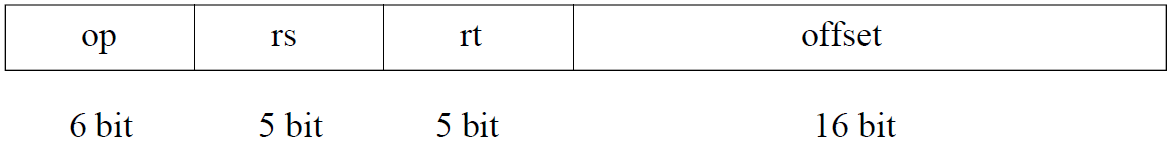
\includegraphics[scale=0.4]{img/loadstore.png}
\caption{Struttura di un'istruzione tipo load/store}\label{fig:loadstore}
\end{figure}
La suddivisione del registro è la seguente:
\begin{description}
\item[op] identifica l'istruzione di tipo load o store
\item[rs] identifica il registro base
\item[rt] identifica il registro sorgente o destinazione per i dati delle operazioni di store o di load da o per la memoria
\item[offset] da sommare all'indirizzo contenuto in \emph{rs} per calcolare l'indirizzo di memoria
\end{description}
\paragraph{Istruzioni di salto}
Per quanto riguarda le istruzioni di salto possiamo suddividerle in due categorie, i salti \emph{condizionati}, che richiedono la verifica di una determinata condizione per decidere se effettuare un salto; oppure istruzioni di salto \emph{incondizionato} che effettuano il salto sempre. 
Lo pseudo assembly di un'istruzione di salto condizionato è:
\begin{verbatim}
beq $s1, $s2, L1	#go to L1 if ($s1 == $s2)
bne $s1, $s2, L1	#go to L1 if ($s1 != $s2)
\end{verbatim}
Le istruzioni di salto condizionato sono nel formato \emph{I-Format}. La suddivisione del registro per questo tipo  di istruzione è mostrata in \figurename\,\ref{fig:condbranch}\\
\begin{figure}[htb]
\centering
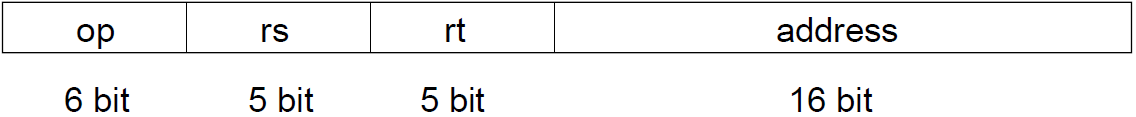
\includegraphics[scale=0.4]{img/condbranch.png}
\caption{Struttura di un'istruzione tipo branch condizionato}\label{fig:condbranch}
\end{figure}
\begin{description}
\item[op] identifica l'istruzione di tipo branch condizionale
\item[rs] identifica il primo registro da comparare
\item[rd] identifica il secondo registro da comparare
\item[address] identifica l'offsett rispetto al PC che corrisponde all'indirizzo dell'etichetta
\end{description}
Per quanto riguarda il salto incondizionato il funzionamento è molto più semplice, quando si raggiunge l'istruzione di salto il PC punta direttamente all'istruzione indicata dall'etichetta. Tale semplicità si rispecchia nella struttura dell'istruzione che in questo caso è di tipo \emph{J-Format}. 
Lo pseudocodice assembly dell'istruzione di salto è:
\begin{verbatim}
j	L1		#go to L1
jr	$s1		#go to add. contenuto in $1
\end{verbatim}
Un esempio di struttura di istruzione di salto è rappresentato in \figurename\,\ref{fig:uncondbranch} 
\begin{figure}[htb]
\centering
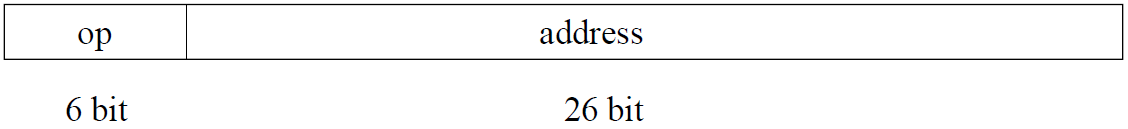
\includegraphics[scale=0.4]{img/uncondbranch.png}
\caption{Divisione delle informazioni in un registro di un istruzione tipo branch incondizionato}\label{fig:uncondbranch}
\end{figure}
dove i valori indicano rispettivamente
\begin{description}
\item[op] identifica il tipo di istruzione
\item[address] identifica l'indirizzo della prossima istruzione da eseguire
\end{description}
Ricapitolando possiamo suddividere le istruzioni in tre categorie in base alla loro struttura e a come vengono eseguite:
\begin{itemize}
\item Tipo R (\emph{Registro})
\begin{itemize}
\item Istruzione ALU
\end{itemize}
\item Tipo I (\emph{Immediate})
\begin{itemize}
\item ALU immediate
\item Istruzioni Load/Store
\item Istruzioni di salto condizionato
\end{itemize}
\item Tipo J (\emph{Jump})
\begin{itemize}
\item Istruzioni di salto incondizionato
\end{itemize}
\end{itemize}
Il perché di questa divisione lo si capisce molto facilmente dallo schema in \figurename\,\ref{fig:rij} nel quale vengono confrontati le diverse suddivisioni degli Instruction Register.
\begin{figure}[htb]
\centering
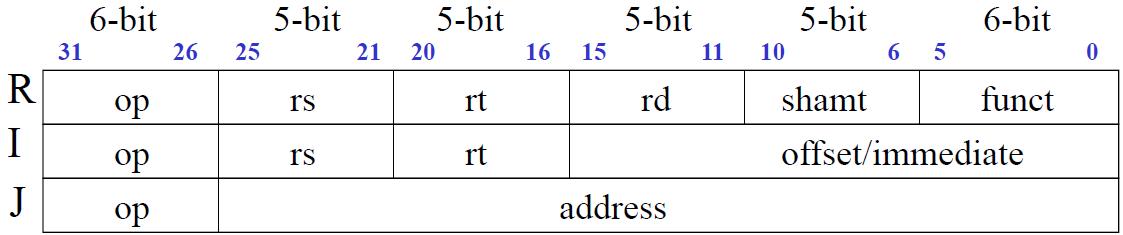
\includegraphics[scale=0.5]{img/rij.png}
\caption{Divisione dei registri nei diversi casi di operazione}\label{fig:rij}
\end{figure}
\subsubsection{Esecuzione delle istruzioni}
Vediamo ora come possono essere implementate le diverse istruzione in ambiente MIPS. Tutte le istruzioni possono essere implementate suddividendo l'esecuzione in cinque fasi distinte:
\begin{enumerate}
\item \textbf{Instruction Fetch Cycle:} durante questo ciclo viene inviato il contenuto del \emph{Program Counter} all'\emph{Instruction Memory} e viene prelevata l'istruzione corrispondente. Successivamente viene aggiornato il PC perchè punti alla prossima istruzione aggiungendo 4 al valore attuale (le istruzioni sono di 4 bytes)
\item \textbf{Instruction Decode and Register Read Cycle:} in questo ciclo si decodifica l'istruzione corrente e si leggono dal \emph{Register File} i registri necessari corrispondenti ai registri specificati nei campi dell'istruzione. Si fa inoltre l'estensione del segno nel caso sia necessario.
\item \textbf{Execution Cycle:} In questo ciclo la ALU effettua le operazioni sugli elementi che sono stati preparati nel ciclo precedente. In base alle istruzioni la ALU esegue le seguenti operazioni
\begin{itemize}
\item Istruzione ALU registro-registro: la ALU esegue le operazioni sugli operandi che ha letto dal \emph{Register File}
\item Istruzioni ALU immediate: la ALU esegue l'operazione specificate sul primo operando letto dal \emph{Register File} e sul operando immediato al quale è stata applicata l'estensione di segno.
\item Istruzioni Load/Store la ALU aggiunge all'indirizzo base l'offset per calcolare l'indirizzo effettivo.
\item Istruzioni di salto condizionato: la ALU compara i due registri e calcola l'indirizzo target del salto da aggiungere al PC
\end{itemize}
\item \textbf{Memory Access (ME):} durante questo ciclo le istruzioni di \emph{Load} effettuano la lettura dalla memoria usando l'indirizzo effettivo calcolato al ciclo precedente, le istruzione di \emph{Store} scrivono nella memoria i dati provenienti dal registro, infine, le istruzioni di \emph{Branch}  aggiornano il valore del Program Counter con l'indirizzo target calcolato al passo precedente, nel caso in cui la condizione sia verificata.
\item \textbf{Write-Back Cycle (WB):} in questo ciclo le istruzioni di \emph{Load} scrivono i dati letti dalla memoria nel registro di destinazione mentre le istruzioni di \emph{ALU} scrivono il risultato delle operazioni nei registri di destinazione.
\end{enumerate}
Come possiamo notare le diverse operazioni non usano sempre tutti i cicli appena descritti ma solitamente (tranne nel caso della \emph{load}) attraversano solo alcune fasi come possiamo vedere dallo schema in \figurename\,\ref{fig:cicli}.\\
Mentre nella tabella di \figurename\,\ref{fig:latency} possiamo vedere le latenze di ogni operazione nel caso di tempo di ciclo uguale ad 1 \emph{ns}.
\begin{figure}[htb]
\centering
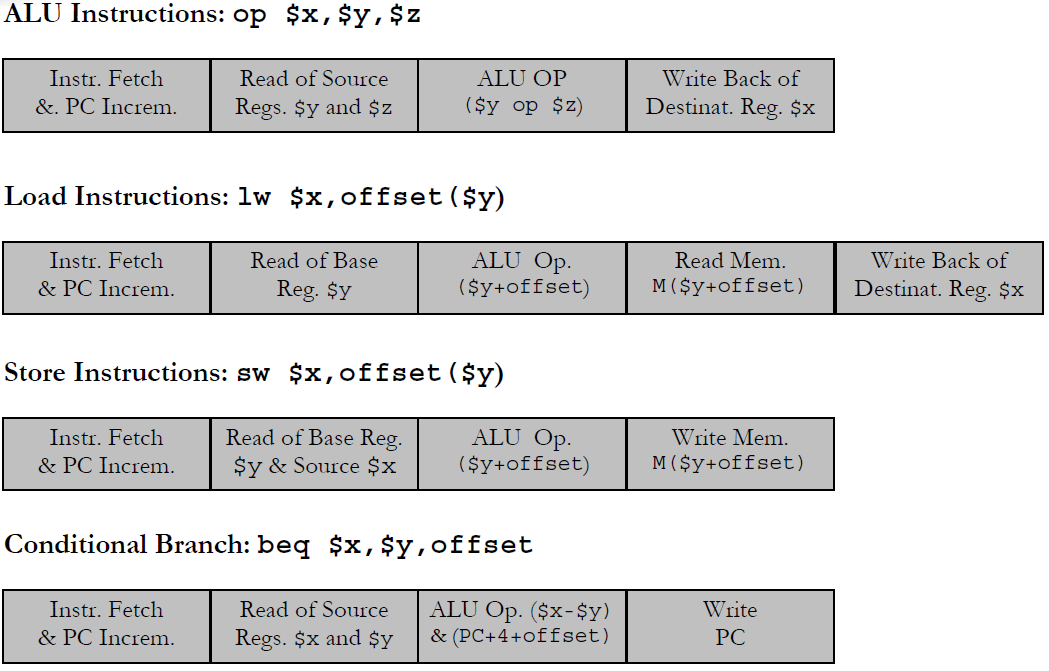
\includegraphics[scale=0.5]{img/cicli.png}
\caption{Cicli eseguiti da ogni operazione}\label{fig:cicli}
\end{figure}
\begin{figure}[htb]
\centering
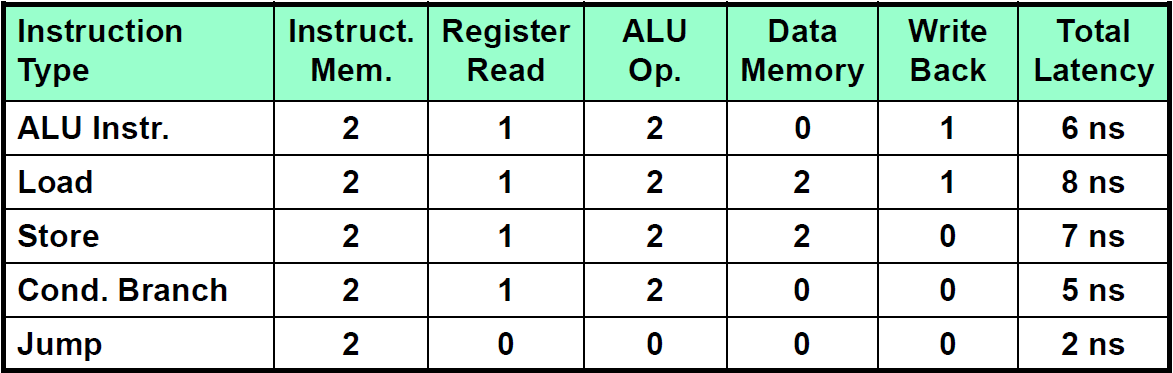
\includegraphics[scale=0.4]{img/latency.png}
\caption{Latenza delle diverse operazioni}\label{fig:latency}
\end{figure}
\subsubsection{Implementazione base di un MIPS}
Vediamo ora come potrebbe essere una semplice implementazione di un \emph{Data Path} in un MIPS. Come notiamo dalla \figurename\,\ref{fig:mips} abbiamo che la parte di memoria dedicata alle istruzioni (\emph{Instruction Memory}) è di sola lettura ed è separata dalla memoria dedicata ai dati (\emph{Data Memory}). Inoltre abbiamo 32 registri organizzati in un \emph{Register File} (RF) con 2 porte di lettura (le due frecce che esco sulla destra) e una porta in scrittura (la freccia in ingresso che punta al campo \emph{Data}).
\begin{figure}[htb]
\centering
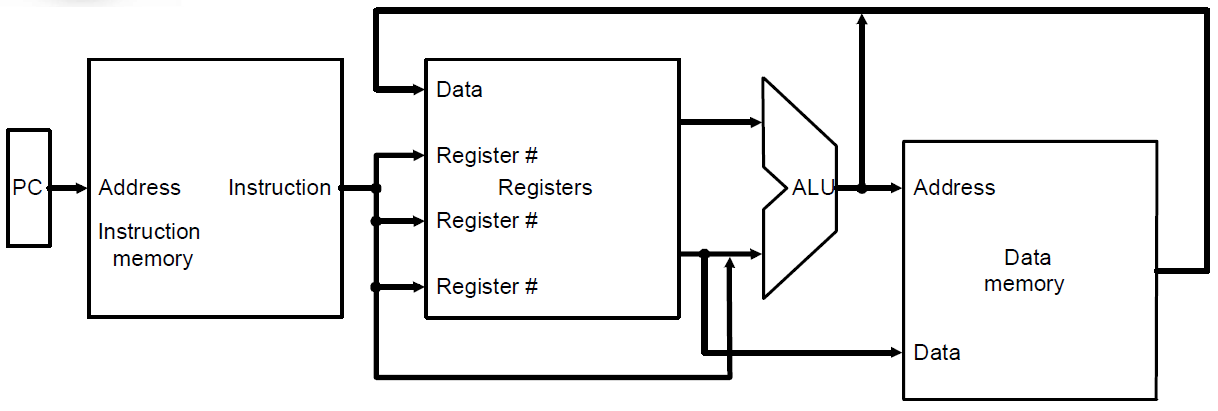
\includegraphics[scale=0.48]{img/mips.png}
\caption{Esempio di implementazione di MIPS}\label{fig:mips}
\end{figure}
La fase di \emph{Instruction Fetch} invece richiede un adder il quale in uscita si connette al PC mentre come ingressi riceve un valore costante \emph{4} mentre all'altro ingresso riceve il valore corrente di del PC come possiamo vedere in \figurename\,\ref{fig:ifetch}.
\begin{figure}[htb]
\centering
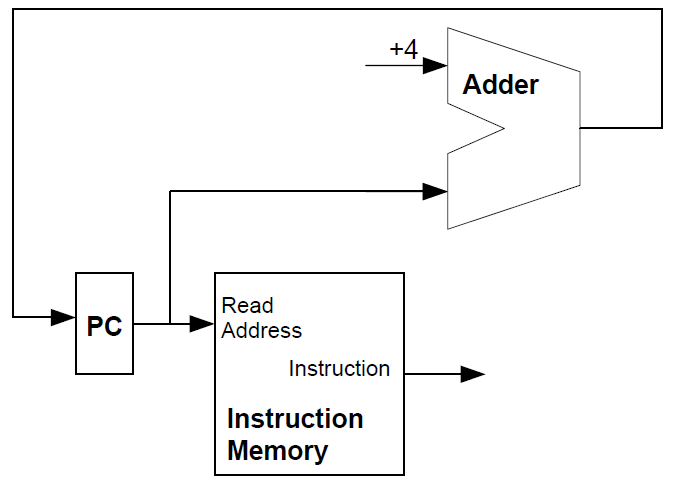
\includegraphics[scale=0.35]{img/ifetch.png}
\caption{Hardware necessario per realizzare l'Instruction Fetch}\label{fig:ifetch}
\end{figure}
Analizziamo ora in breve quale hardware è necessario per implementare le diverse operazioni che possono essere eseguite da un MIPS. Partiamo con l'analizzare un istruzione di tipo ALU come vediamo in \figurename\,\ref{fig:ALUhw}. Dal \emph{Register File} escono due porte che sono connesse ad un'unità ALU la quale ha un uscita \emph{Result} che si connette alla porta di scrittura del \emph{RF} e un'uscita \emph{Zero} per indicare eventuali anomalie. Inoltre la ALU ha un ingresso \emph{OP} che serve a selezionare il tipo di operazione.
\begin{figure}[htb]
\centering
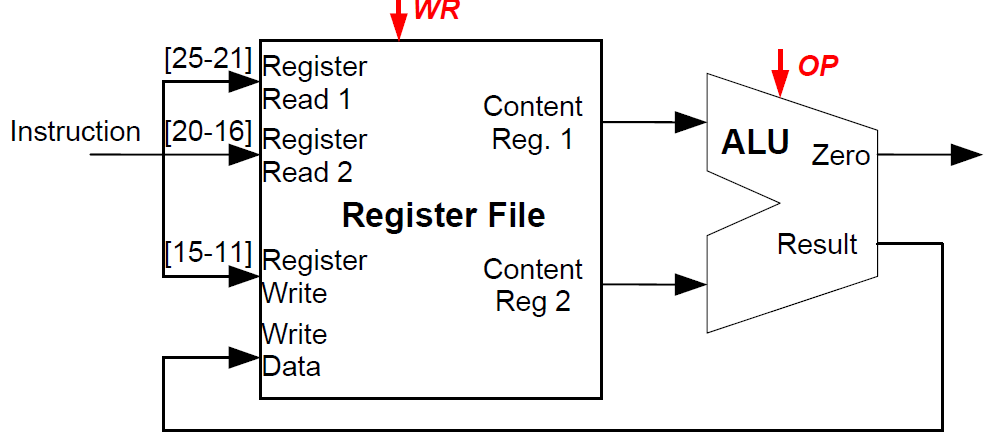
\includegraphics[scale=0.4]{img/aluhw.png}
\caption{Hardware che implementa un istruzione di tipo aritmetico}\label{fig:ALUhw}
\end{figure}
Per quanto riguarda l'istruzione di \emph{load} e quella di \emph{store} sono molto simili come si può vedere da \figurename\,\ref{fig:loadhw} e da \figurename\,\ref{fig:storehw}. Nel caso della load la alu calcola l'indirizzo di memoria da leggere il quale viene inviato alla memoria e il risultato della lettura è registrato tramite la porta write data del \emph{RF}. Nel caso della \emph{store} invece la ALU calcola l'indirizzo di destinazione della scrittura e tramite la porta write del \emph{Data Memory} viene copiato il valore del registro.
\begin{figure}[htb]
\centering
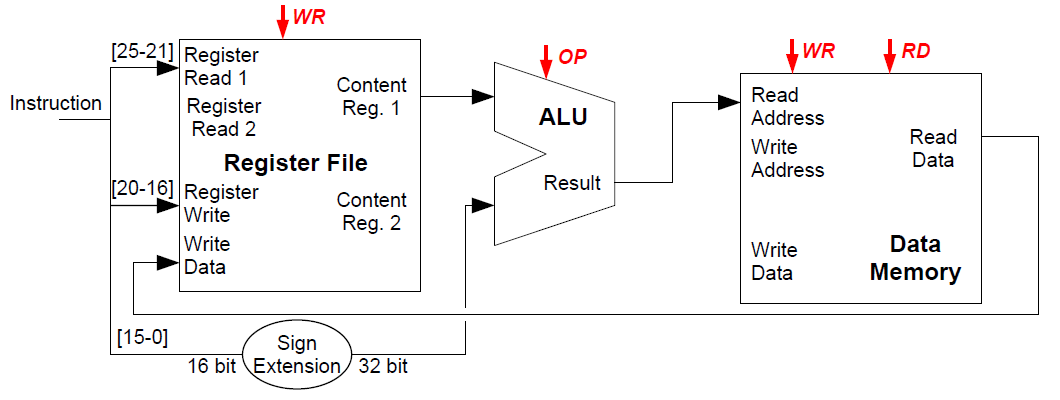
\includegraphics[scale=0.45]{img/loadhw.png}
\caption{Hardware che implementa un istruzione di tipo load}\label{fig:loadhw}
\end{figure}
\begin{figure}[htb]
\centering
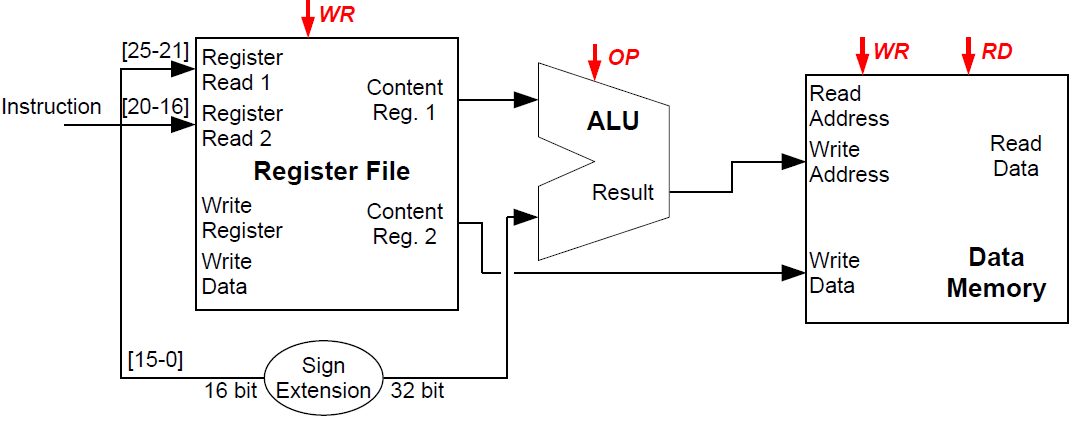
\includegraphics[scale=0.45]{img/storehw.png}
\caption{Hardware che implementa un istruzione di tipo store}\label{fig:storehw}
\end{figure}
In entrambi i casi un unità particolare si occupa di eseguire l'estensione del segno in caso di bisogno.\\
Stabiliamo ora come viene implementato il clock del circuito; possiamo avere due possibilità, la prima è avere un unico ciclo di clock lungo quanto il percorso critico necessario per eseguire l'istruzione di load (la più lunga), la seconda è avere un ciclo di clock lungo quanto un singolo passaggio in uno dei componenti prima analizzati.\\
Analizziamo innanzitutto il caso di singolo ciclo, in questo caso il ciclo dovrà avere una durata pari al tempo necessario per eseguire un'istruzione di load che come abbiamo visto è pari a $T = 8 ns \quad (f=125 \ MHz)$. Assumiamo quindi che ogni istruzione verrà eseguita in un singolo ciclo di clock, ogni modulo verrà utilizzato una sola volta per clock e quei moduli che dovrebbero essere utilizzati più di una volta dovranno essere duplicati.
Inoltre dobbiamo tener conto anche delle differenze tra i diversi tipi di istruzioni, infatti, all'ingresso di scrittura dell'RF possiamo avere dati provenienti da una ALU e quindi di lunghezza [15-11] bit oppure dati provenienti da una load/store con una lunghezza di [20-16] bit questo richiede un \emph{Multiplexer} all'ingresso dei registri nel RF. In secondo luogo al secondo ingresso della ALU possiamo avere avere il dato proveniente da un registro nel caso di operazioni ALU oppure l'offset per le istruzioni di load/store, questo richiede un \emph{MUX} al secondo ingresso della ALU. Infine i dati all'output del Destination Register possono arrivare sia dal risultato della ALU oppure dal Data Memory nel caso di load questo comporta l'utilizzo di un \emph{MUX} all'ingresso in scrittura dei dati su RF.
In \figurename~\ref{fig:monocic} vediamo l'implementazione completa di un MIPS a ciclo singolo con l'introduzione, oltre che dei MUX precedentemente specificati, anche di una ALU (parte alta della figura) che permette l'implementazione dei branch, e della logica di controllo (in rosso nella figura)\\
Veniamo ora al caso in cui il ciclo di clock sia di lunghezza pari al tempo necessario per un singolo modulo $T = 2 ns$ questo significa che per eseguire un'istruzione di load sono necessari 5 cicli di clock per un totale di \emph{10ns}. Ogni fase dell'istruzione richiede un ciclo di clock ma questo permette la condivisione dei moduli tra diverse istruzioni in differenti cicli di clock, anche se questo richiede l'inserimento di registri tra un'unità  e l'altra.
\begin{figure}[!Hptb]
\centering
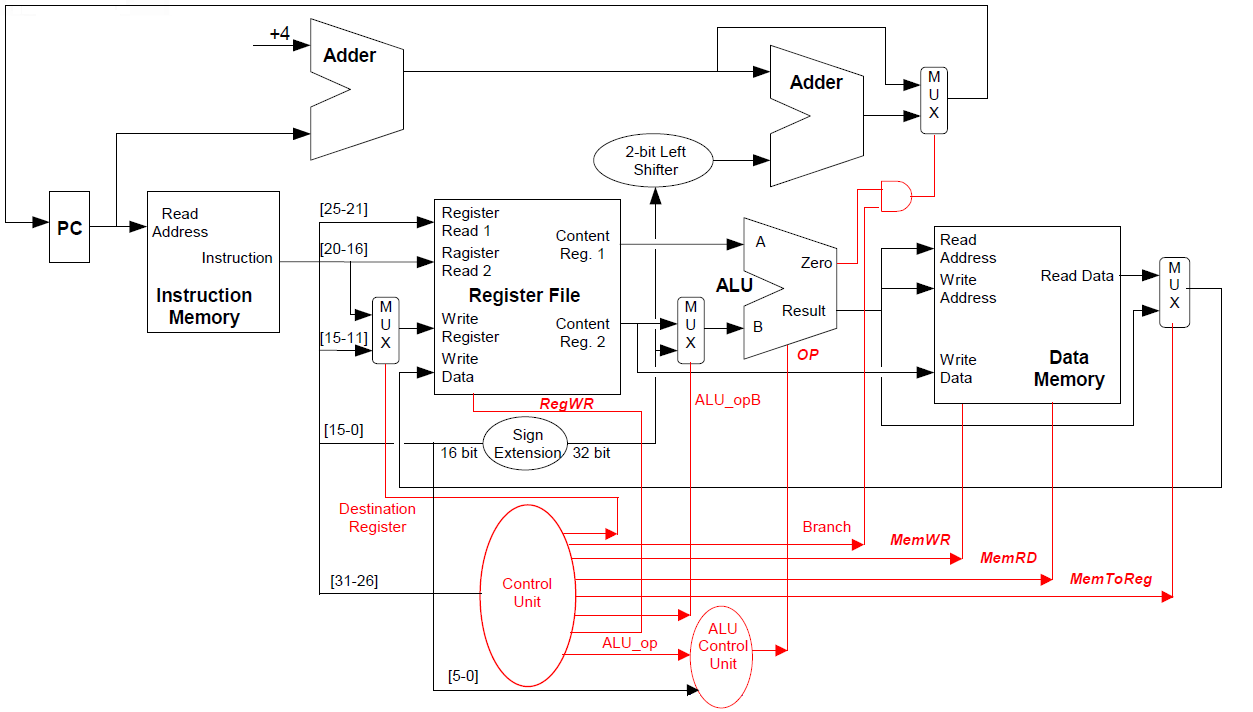
\includegraphics[scale=0.67, angle=90]{img/monocic.png}
\caption{MIPS a singolo ciclo con logica di controllo}\label{fig:monocic}
\end{figure}
\subsection{Pipelining}
Il pipelining è una tecnica di ottimizzazione basata sull'esecuzione multipla sovrapposta di istruzioni sequenziali. L'idea fondamentale è quella di sfruttare il parallelismo intrinseco delle istruzioni sequenziali in quanto l'esecuzione di una istruzione è suddivisa in fasi differenti (\emph{pipelines stages}) che richiedono soltanto una piccola frazione di tempo per essere completate. I diversi stati sono connessi in sequenza nella pipeline, un'istruzione entra da una parte procede attraverso i diversi stadi e esce all'altro capo come in una catena di montaggio.\\
I vantaggi di questa tecnica è che è completamente trasparente al programmatore, inoltre come in una catena di montaggio, il tempo necessario per eseguire un'istruzione è uguale al caso in cui l'istruzione sia eseguita senza pipeline; quello che la pipeline fa è incrementare il numero di istruzioni eseguite contemporaneamente e perciò aumentare la frequenza di completamento come vediamo in \figurename\,\ref{fig:seqvspipe}\\
\begin{figure}[tb]
\centering
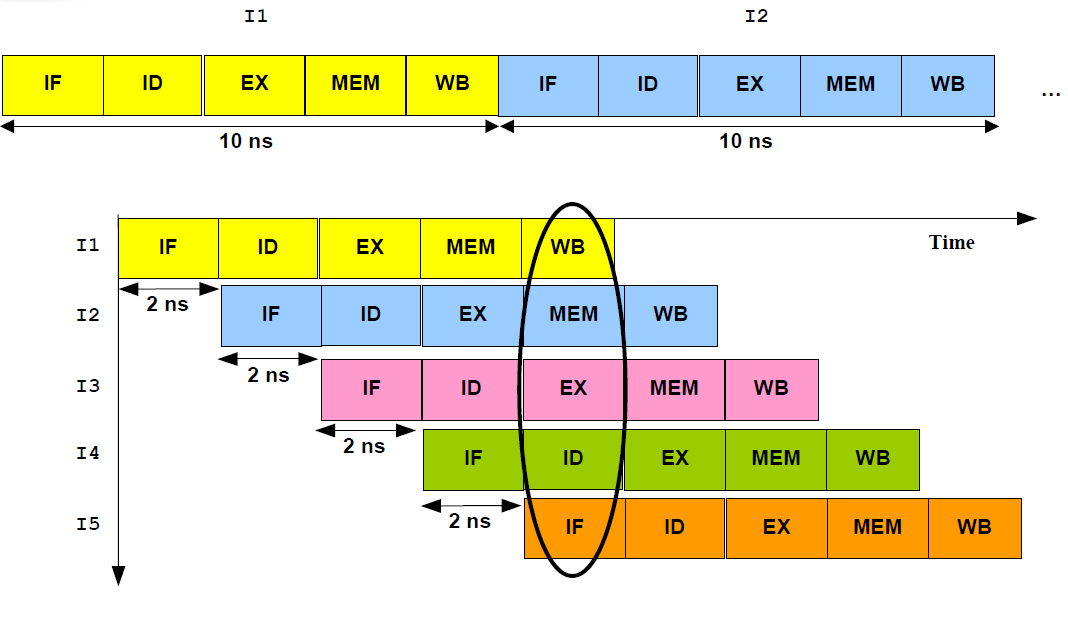
\includegraphics[scale=0.4]{img/seqvspipe.png}
\caption{Confronto tra esecuzione sequenziale e pipelined}\label{fig:seqvspipe}
\end{figure}
Il tempo necessario per far avanzare un'istruzione di una fase corrisponde ad un ciclo di clock, le diverse fasi perciò devono essere \emph{sincronizzate}, il periodo di clock deve essere uguale al tempo di esecuzione della fase più lenta (nel nostro esempio 2ns). L'obiettivo è quello di bilanciare la lunghezza di ogni fase della pipeline in modo da avere uno \emph{speedup ideale} uguale al numero di fasi della pipeline.\\
Nel caso ideale vediamo come la pipeline sia più efficiente sia dell'architettura a singolo ciclo che a quella multi-ciclo viste in precedenza.
Nel caso di una CPU1 non pipeline con un unico ciclo di clock della durata di 8ns contro una CPU2 con una pipeline a 5 stadi e ciclo di 2ns abbiamo che:
\begin{itemize}
\item la \emph{latenza} ovvero il tempo necessario per eseguire una istruzione è peggiore nel caso di CPU2: 8ns vs 10ns
\item il \emph{throughput} tuttavia è notevolmente migliorato: $1 \ istruzione/8ns$ vs $1 \ istruzione/2ns$
\end{itemize}
Nel caso di CPU3 multi-ciclo senza pipeline contro un'architettura CPU2 come quella descritta in precedenza abbiamo:
\begin{itemize}
\item la \emph{latenza} resta invariata: 10 ns
\item il \emph{throughput} cresce di ben 5 volte: $1 \ istruzione/10ns$ vs $1 \ istruzione/2ns$
\end{itemize}
\subsubsection{Implementazione di una Pipeline}
Innanzitutto vediamo quali fasi devono attraversare ciascuna operazione in quanto non tutte le fasi sono necessarie per tutte le operazioni, uno schema riassuntivo è specificato in \figurename\,\ref{fig:pipefasi}.\\
\begin{figure}[tbh]
\centering
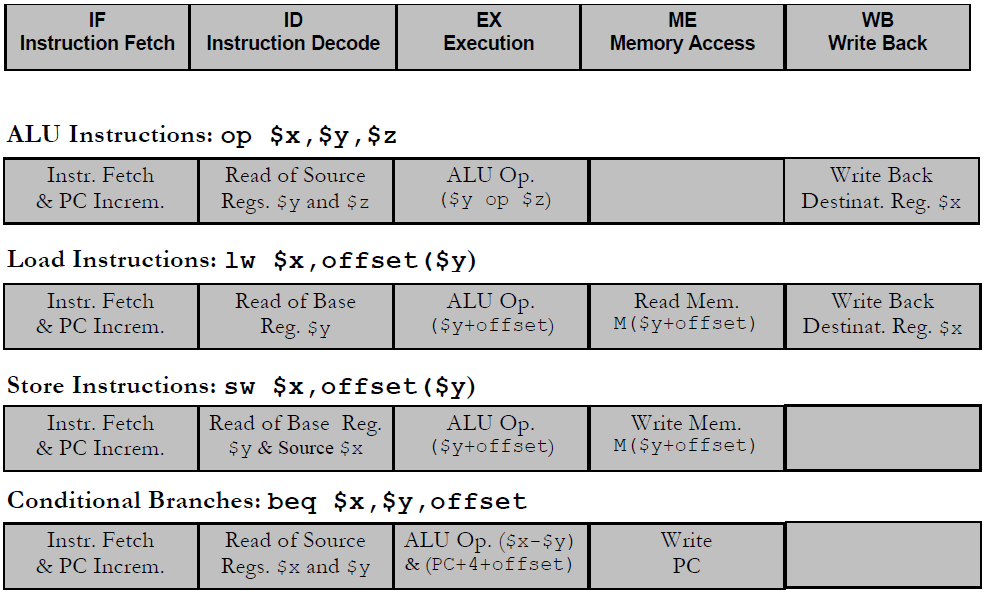
\includegraphics[scale=0.4]{img/pipefasi.png}
\caption{Fasi della pipeline necessarie ad ogni istruzione}\label{fig:pipefasi}
\end{figure}
La divisione dell'esecuzione di una istruzione in 5 fasi implica che in ogni ciclo di clock cinque istruzione sono in esecuzione questo comporta la necessità di inserire dei \emph{registri} tra una fase e l'altra della pipeline per separare i diversi stage.\\
In \figurename\,\ref{fig:pipeline} vediamo una possibile implementazione di un'architettura MIPS pipelined con l'introduzione dei registri tra le fasi (in verde).
\begin{figure}[!Hptb]
\centering
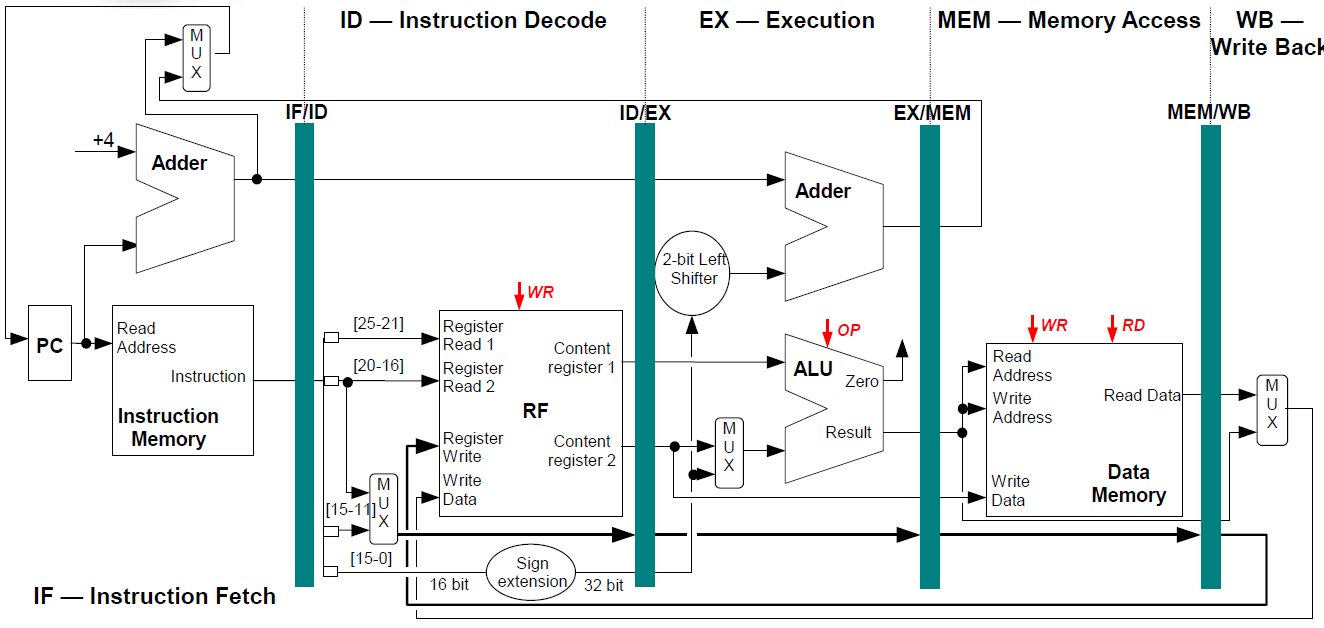
\includegraphics[scale=0.6, angle=90]{img/pipeline.png}
\caption{Schema di un MIPS con pipeline}\label{fig:pipeline}
\end{figure}
\pagebreak
\subsection{Il problema del ''Hazard''}
Si ha un \emph{hazard} quando vi è una dipendenza tra istruzioni diverse e la sovrapposizione dovuta al pipeline cambia l'ordine di dipendenza sugli operandi. Hazard previene l'esecuzione della prossima istruzione nel ciclo di clock designato ma così facendo riduce le performance allontanandole dallo speedup ideale.\\
Possiamo distinguere tre classi di \emph{hazard}:
\begin{itemize}
\item \textbf{Structural Hazards:} si ha quando diverse istruzioni cercano di utilizzare la stessa risorsa simultaneamente (stessa memoria per istruzioni e dati)
\item \textbf{Data Hazards:} si ha quando si cerca di utilizzare un risultato prima che questo sia pronto(istruzione dipendente dalla precedente che è nella pipeline)
\item \textbf{Control Hazards:} si ha quando si deve prendere una decisione sulla esecuzione della prossima istruzione prima della valutazione di una condizione (branch condizionali)
\end{itemize}
Tra questi tre tipi di hazard il primo non può presentarsi nelle architetture MIPS in quanto lo spazio di memoria dedicato alle istruzioni e quello dedicato ai dati sono fisicamente separati.
\subsubsection{Data Hazard}
Per quanto riguarda il data hazard si verifica quando sono in esecuzione nella pipeline due o più istruzioni \emph{dipendenti}.
\begin{verbatim}
sub   $2, $1, $3
and   $12, $2, $5   #1° operando dipende dalla sub
or    $13, $6, $2   #2° operando dipende dalla sub
add   $14, $2, $2   #1° & 2° operando dipendono dalla sub
sw    $15, 100($2)  #Il registro base dipende dalla sub
\end{verbatim}
Come vediamo dall'esempio qui sopra e dalla sua esecuzione in \figurename\,\ref{fig:datahazard} abbiamo che le istruzioni successive alla \texttt{sub} debbono aspettare che la prima istruzione arrivi nella fase di \emph{write-back} prima di poter utilizzare il dato come avviene per l'ultima istruzione evidenziata da una freccia verde.
\begin{figure}[htb]
\centering
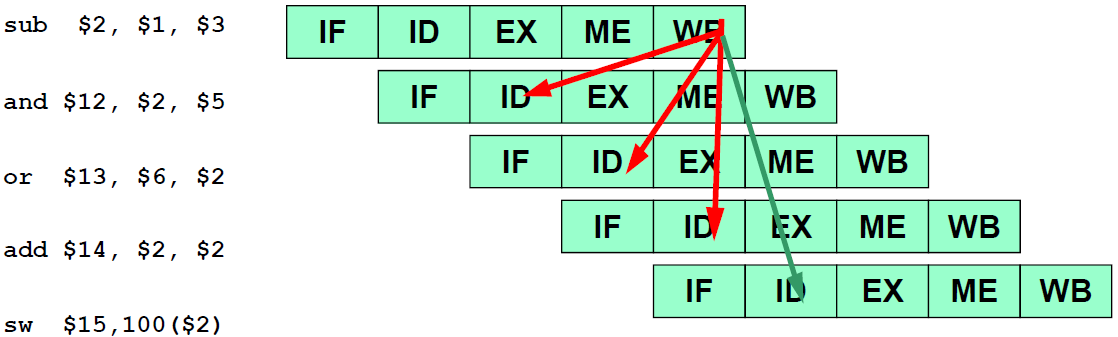
\includegraphics[scale=0.5]{img/datahazard.png}
\caption{Esempio di data hazard}\label{fig:datahazard}
\end{figure}
Esistono diversi meccanismi per far si che queste dipendenze vengano soddisfatte, le principali si possono suddividere in due categorie:
\begin{itemize}
\item \textbf{Tecniche di compilazione:} in questa categoria rientra il re-scheduling delle operazioni che connsiste nell'inserire istruzioni indipendenti tra le istruzioni correlate in modo da permettere il calcolo dei valori necessari; nel caso non sia possibile inserire altre operazioni il compilatore inserisce delle \texttt{nop} ovvero delle operazioni che non fanno nulla \emph{no operation}
\item \textbf{Tecniche hardware:} in questa categoria rientrano la possibilità di inserire delle \emph{bubbles} o degli stalli oppure le tecniche di \emph{Data Forwarding} e di \emph{Bypassing}
\end{itemize}
Vediamo innanzi tutto un esempio di inserimento di \texttt{nop} in \figurename\,\ref{fig:nop}
\begin{figure}[htb]
\centering
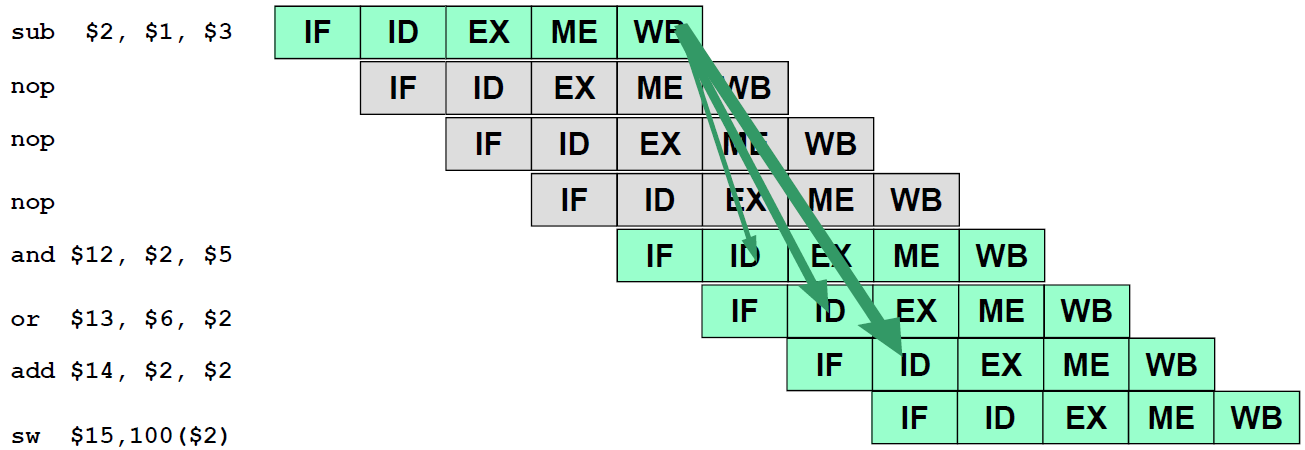
\includegraphics[scale=0.45]{img/nop.png}
\caption{Esempio di uso \texttt{nop}}\label{fig:nop}
\end{figure}
Come vediamo l'inserimento di nop perggiora lo speedup ideale, cosa che invece non succede se si applicano le tecniche di re-scheduling in quanto non vengono inserite istruzioni inutili nell'esecuzione  delle istruzioni ma viene modificato semplicemente l'ordine nel quale vengono eseguite.\\
Il caso di inserimento di stalli è molto simile a quello di inserimento delle nop la differenza sta nel fatto che si ferma l'esecuzione dell'istruzione dipendente il tempo necessario affinché l'istruzione in esecuzione renda disponibile il dato come vediamo in \figurename\,\ref{fig:stall}, anche in questo caso abbiamo un peggioramento dello speedup ideale.
\begin{figure}[htb]
\centering
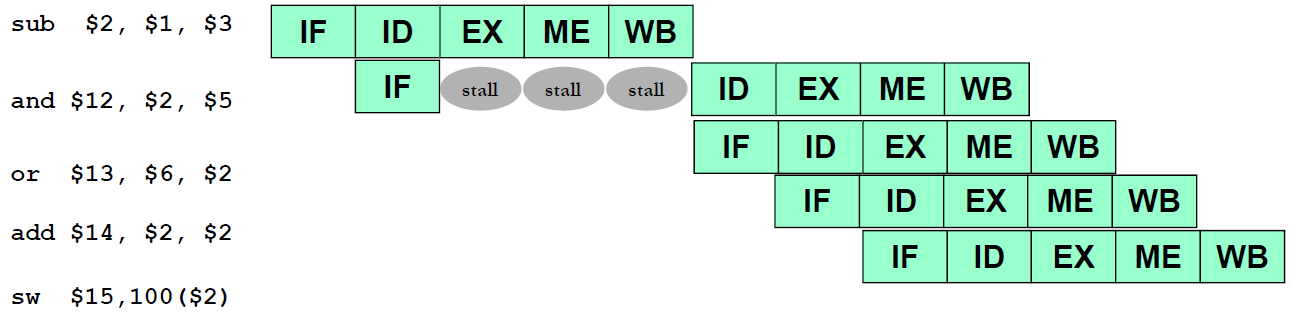
\includegraphics[scale=0.45]{img/stall.png}
\caption{Esempio di uso degli stalli}\label{fig:stall}
\end{figure}
\paragraph{Data Forwarding}
Il \emph{data forwarding} è una tecnica hardware che comporta l'utilizzo dei risultati temporanei immagazzinati nei registri della pipeline, per fare ciò abbiamo bisogno di aggiungere dei \emph{multiplexer} all'ingresso della ALU per selezionare la provenienza dei dati. In \figurename\,\ref{fig:forwardingpath} vediamo quali sono i collegamenti necessari per l'esecuzione di istruzioni aritmetiche dipendenti; questi path sono tre:
\begin{itemize}
\item\textbf{EX/EX path:} in figura da ALU ad ALU che risolve il problema di due istruzioni consecutive nella quale la seconda necessita del risultato della prima. Nell'esempio precedente la dipendenza \texttt{sub}$\rightarrow$\texttt{and}
\item\textbf{MEM/EX path:} in questo caso si risolve la dipendenza tra la prima e la terza istruzione (\texttt{sub}$\rightarrow$\texttt{or})
\item\textbf{MEM/ID path:} risolve la dipendenza tra la prima e la quarta istruzione (\texttt{sub}$\rightarrow$\texttt{add})
\end{itemize}
Con l'introduzione di questi path si riesce a risolvere tutti i problemi di dipendenza per quanto riguarda le istruzioni di tipo aritmetico.
In \figurename\,\ref{fig:forwardingcirc} vediamo una possibile implementazione hardware di una pipeline con sistema di forwarding path.
\begin{figure}[htb]
\centering
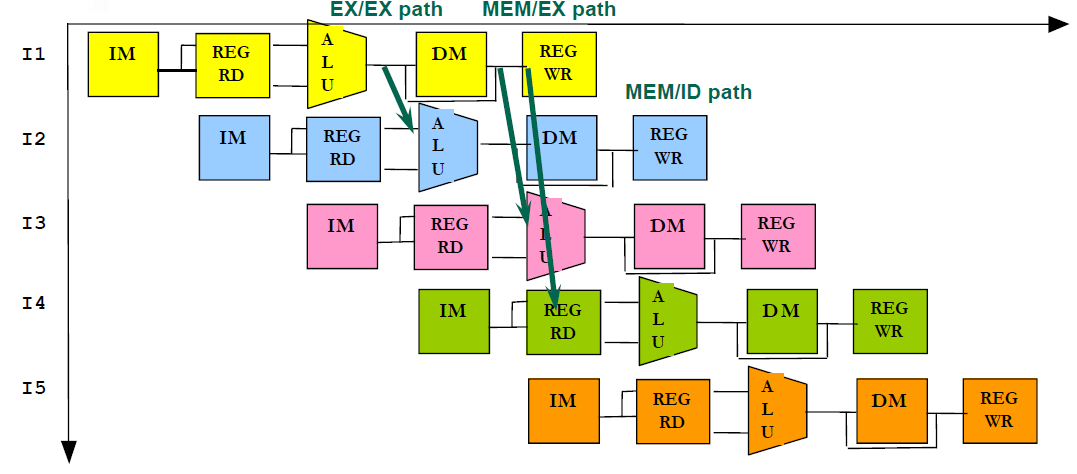
\includegraphics[scale=0.45]{img/forwardingpath.png}
\caption{Esempio di forwarding path}\label{fig:forwardingpath}
\end{figure}
\begin{figure}[htb]
\centering
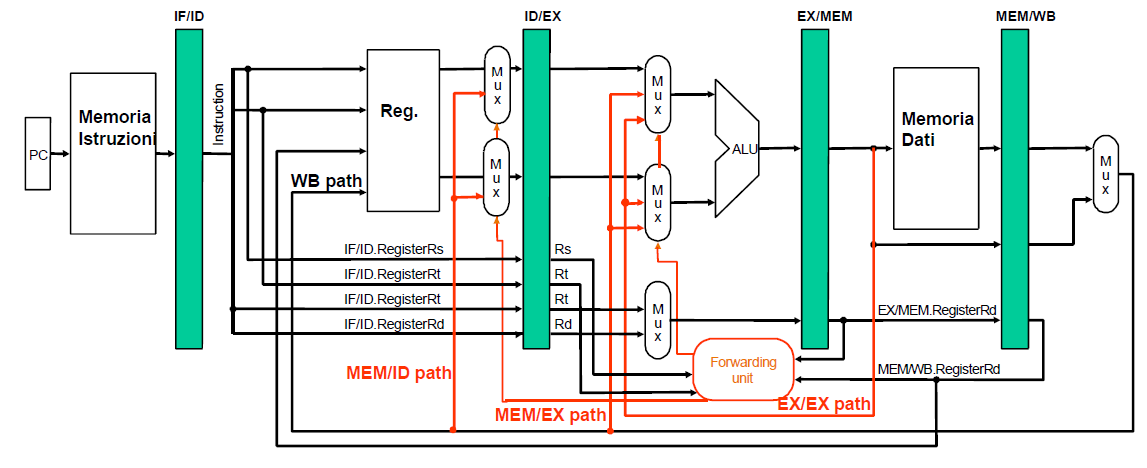
\includegraphics[scale=0.7,angle=90]{img/forwardingcirc.png}
\caption{Schema MIPS con forwarding}\label{fig:forwardingcirc}
\end{figure}
Esiste ancora una situazione però in cui è necessario inserire degli stalli, questa situazione è dovuta alla sequenza di istruzioni seguenti:
\begin{verbatim}
L1: lw  $s0, 4($t1)     #$s0<-M[4 + $t1]
L2: add $s5, $s0, $s1   #1° operand depends from L1
\end{verbatim}
Questa dipendenza si crea in quanto il dato viene scritto in \texttt{\$s0} solo nella fase di WB mentre viene letto durante la fase di ID. In questo caso non si può fare molto se non sfruttare il forwarding path MEM/EX già analizzato prima anche se comunque è necessario introdurre uno stallo per risolvere la dipendenza.
Nel caso invece in cui la dipendenza sia tra un'istruzione di \emph{load} e una di \emph{store} si può risolvere la dipendenza aggiungendo un \emph{forwarding path} tra le due fasi di MEM. Questo path permette di risolvere la dipendenza senza dover introdurre altri stalli come si può vedere in \figurename\,\ref{fig:memmempath}.
\begin{figure}
\centering
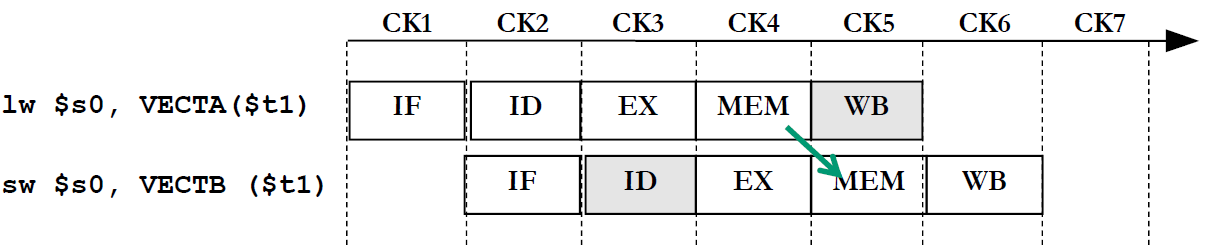
\includegraphics[scale=0.5]{img/memmempath.png}
\caption{Forwarding path tra due fasi di memorizzazione successive.}\label{fig:memmempath}
\end{figure}
Con l'architettura attuale, come abbiamo visto, nel caso di dipendenza tra una \emph{load} ed un'istruzione aritmetica che legge un registro è necessario introdurre uno stallo; in quanto l'accesso in lettura avviene durante la fase di ID mentre la scritture avviene durante la fase di WB. Nel caso, invece, di \emph{pipeline ottimizzata} possiamo assumere che la fase di lettura avviene nelle seconda metà del ciclo di clock mentre la fase di scrittura nella prima metà; in questo modo nel caso in cui lettura e scrittura facciano riferimento allo stesso registro nello stesso ciclo di clock non è più necessario inserire degli stalli, e si può inoltre eliminare il forwarding path tra MEM e ID.
\subsubsection{Altri tipi di Data Hazard}
Fino ad ora abbiamo analizzato solo un tipo di dipendenza sui dati, questo tipo di dipendenza è chiamato \textbf{RAW (Read After Write)}, e si ha quando l'istruzione \emph{n+1} cerca di leggere un registro prima che l'istruzione n abbia finito di scrivere tale registro.\\
Esistono tuttavia altri due tipi di \emph{data hazard} che sono:
\begin{itemize}
\item Write After Write (WAW)
\item Write After Read (WAR)
\end{itemize}
La dipendenza di tipo WAW si ha quando un istruzione n+1 di tenta di scrivere un registro il quale non è ancora stato scritto dall'istruzione n. Tale tipo di dipendenza avviene solo nel caso in cui la nostra pipeline preveda la possibilità di fasi di memorizzazione o di esecuzione multi-ciclo come mostrato in \figurename\,\ref{fig:multimem} e \ref{fig:multiexe} le quali portano alla terminazione delle istruzione fuori ordine
\begin{figure}
\centering
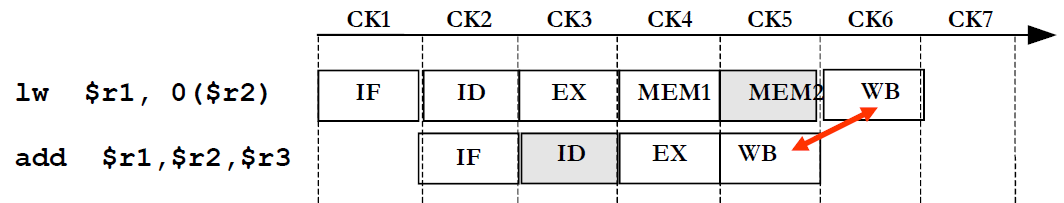
\includegraphics[scale=0.4]{img/multimem.png}
\caption{Fase di memorizzazione multiciclo che porta alla creazione di dipendenze di tipo WAW}\label{fig:multimem}
\end{figure}
\begin{figure}
\centering
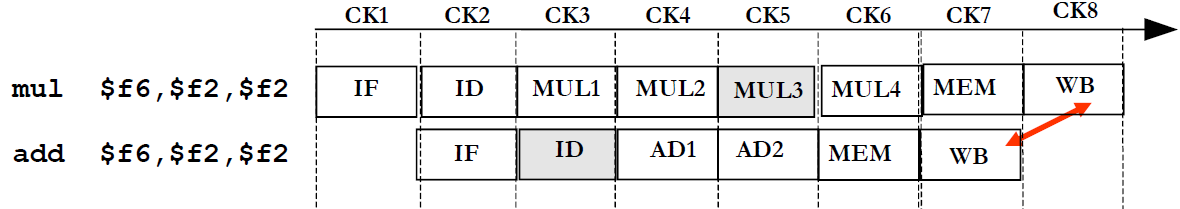
\includegraphics[scale=0.4]{img/multiexe.png}
\caption{Fase di esecuzione multiciclo che porta alla creazione di dipendenze di tipo WAW}\label{fig:multiexe}
\end{figure}
Per quanto riguarda le dipendenze di tipo WAR si hanno quando l'istruzione n+1 tenta di scrivere un registro prima che questo sia stato letto da un istruzione n, nel caso di architettura MIPS però tale tipo di dipendenza non può mai verificarsi in quanto la lettura avviene nella fase ID mentre la scrittura nella fase WB.
\subsection{Analisi delle performance}
L'utilizzo della pipeline aumenta il throughput della CPU ma non riduce il tempo di esecuzione della singola istruzione, anzi solitamente aumenta la latenza di ogni istruzione bisogna quindi bilanciare il numero di fasi con l'overhead dovuto alla pipeline.\\
Definito $IC = Instruction \ Count$ ovvero il numero di istruzioni eseguite, possiamo determinare il numero di cicli di clock necessari per completare queste operazioni operazione. Tale valore è uguale a:
$$\#Clock \ Cycle = IC + \# Stall \ Cycles + 4$$
Dividendo tale valore per il numero di operazioni otteniamo:
$$
\begin{array}{rcl}
CPI & = &Clock \ Per \ Instruction = \# Clock \ Cycle /IC = \\
& = & (IC + \#Stall \ Cycles + 4)/IC
\end{array}
$$
$$MIPS= f_{clock} / (CPI * 10^6)$$
Come visto fino ad ora la CPI ideale per la pipeline è 1 ma gli stalli degradano le performance.
Abbiamo così che la CPI media è data da:
$$
\begin{array}{rcl}
Ave. \ CPI & = & Ideal \ CPI + \#Stall \ per \ Instruction \\
& = & 1 + \#Stall \ per \ Instruction
\end{array}
$$
Possiamo misurare il miglioramento delle performance dato dall'introduzione della pipeline come
$$
\begin{array}{rcl}
Pipeline \ SpeedUp & = & \frac{Ave. \ Exec. \ Time \ Unpipelined}{Ave. \ Exec. \ Time \ Pipelined} = \\
& = & \frac{Ave. \ CPI \ Unp.}{Ave. \ CPI \ Pipe} \times \frac{Clock \ Cycle \ Unp.}{Clock \ Cycle \ Pipe}
\end{array}
$$
Se ignoriamo l'overhead sul tempo di clock e assumiamo che i diversi stage siano perfettamente bilanciati possiamo ridefinire lo speedup come
$$SpeedUp_{pipeline} = \frac{Ave. \ CPI \ Unp.}{1 + \# Stall \ per \ Instruction}$$
Nel caso ideale nel quale tutte le istruzioni richiedano lo stesso numero di cicli questi sono uguali al numero di fasi della pipeline e possiamo riscrivere la precedente come:
$$SpeedUp_{pipeline} = \frac{Pipeline \ Depth}{1 + \# Stall \ per \ Instruction}$$
Nel caso ideale in cui non ci siano stalli vediamo come le performance migliori tanto è più profonda (maggior numero di fasi) la pipeline.\\
Nel caso in cui si abbiano dei salti condizionati le performance peggiorano in base alla penalità del branch, infatti:
$$SpeedUp_{pipeline} = \frac{Pipeline \ Depth}{1 + Branch \ Frequency \times Branch \ Penalty}$$

